\documentclass[12pt,a4paper,twoside]{article}
\usepackage{graphicx}

\setlength{\parindent}{0cm}
\setlength{\parskip}{2ex plus1ex minus 0.5ex}

\addtolength{\evensidemargin}{-2.5cm}
\addtolength{\oddsidemargin}{-1cm}
\addtolength{\textwidth}{3cm}
\addtolength{\topmargin}{-3.5cm}
\addtolength{\textheight}{3.5cm}

% \newcommand{\source}[1]{\textbf{\verb^#1^}}}
\newcommand{\mission}[1]{\item[#1:]}

\pagestyle{empty}
\input{macros}

\begin{document}
\ \\[1cm]
{
\huge \sffamily
\begin{center}
\textbf{Roboc practical exercises}\\[9mm]
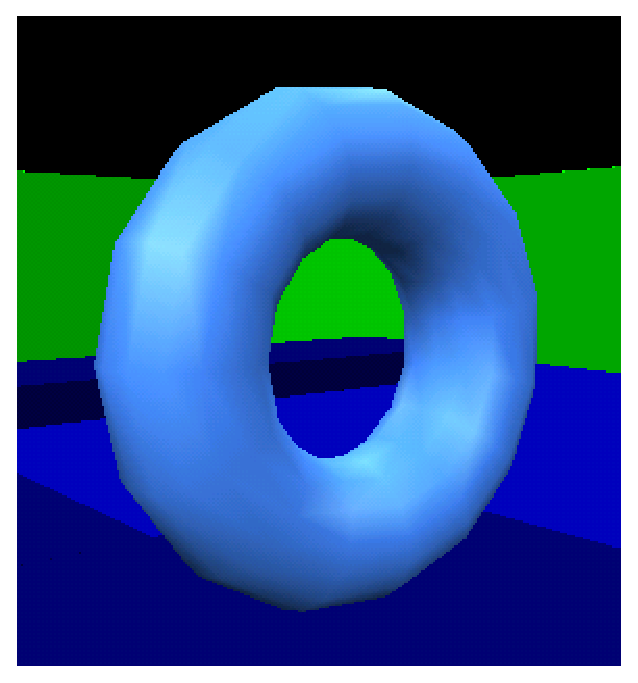
\includegraphics[scale=0.5,angle=0]{screenshots/3d/torus}
\\[6mm]
%3D Graphics\\
% Royal Institution Mathematics Masterclass\\
% 2nd Feb 2008

Sutton Trust Summer School\\
August 2010
% Roboc V7\\[-2mm]

% Dr DM Ingram, University of Cambridge
\end{center}
\vspace{30mm}

\begin{tabular}{rl}
\textbf{Name:} & \framebox[10cm]{\rule[-5mm]{0mm}{15mm}}\\[20mm]
\textbf{Login ID:} & v3490\\[20mm]
\textbf{Password:} & staug10
\end{tabular}
}
\end{document}
